\documentclass{standalone}
\usepackage{tikz}
\usepackage{adjustbox}
\usepackage{helvet}  
\usepackage{sansmathfonts}  
\renewcommand{\familydefault}{\sfdefault}  
\usetikzlibrary{arrows.meta,calc,decorations.pathmorphing}
\usetikzlibrary{shapes.geometric, shapes.arrows}
\usepackage[svgnames]{xcolor}

\definecolor{colorFFFFFF}{HTML}{FFFFFF}
\begin{document}
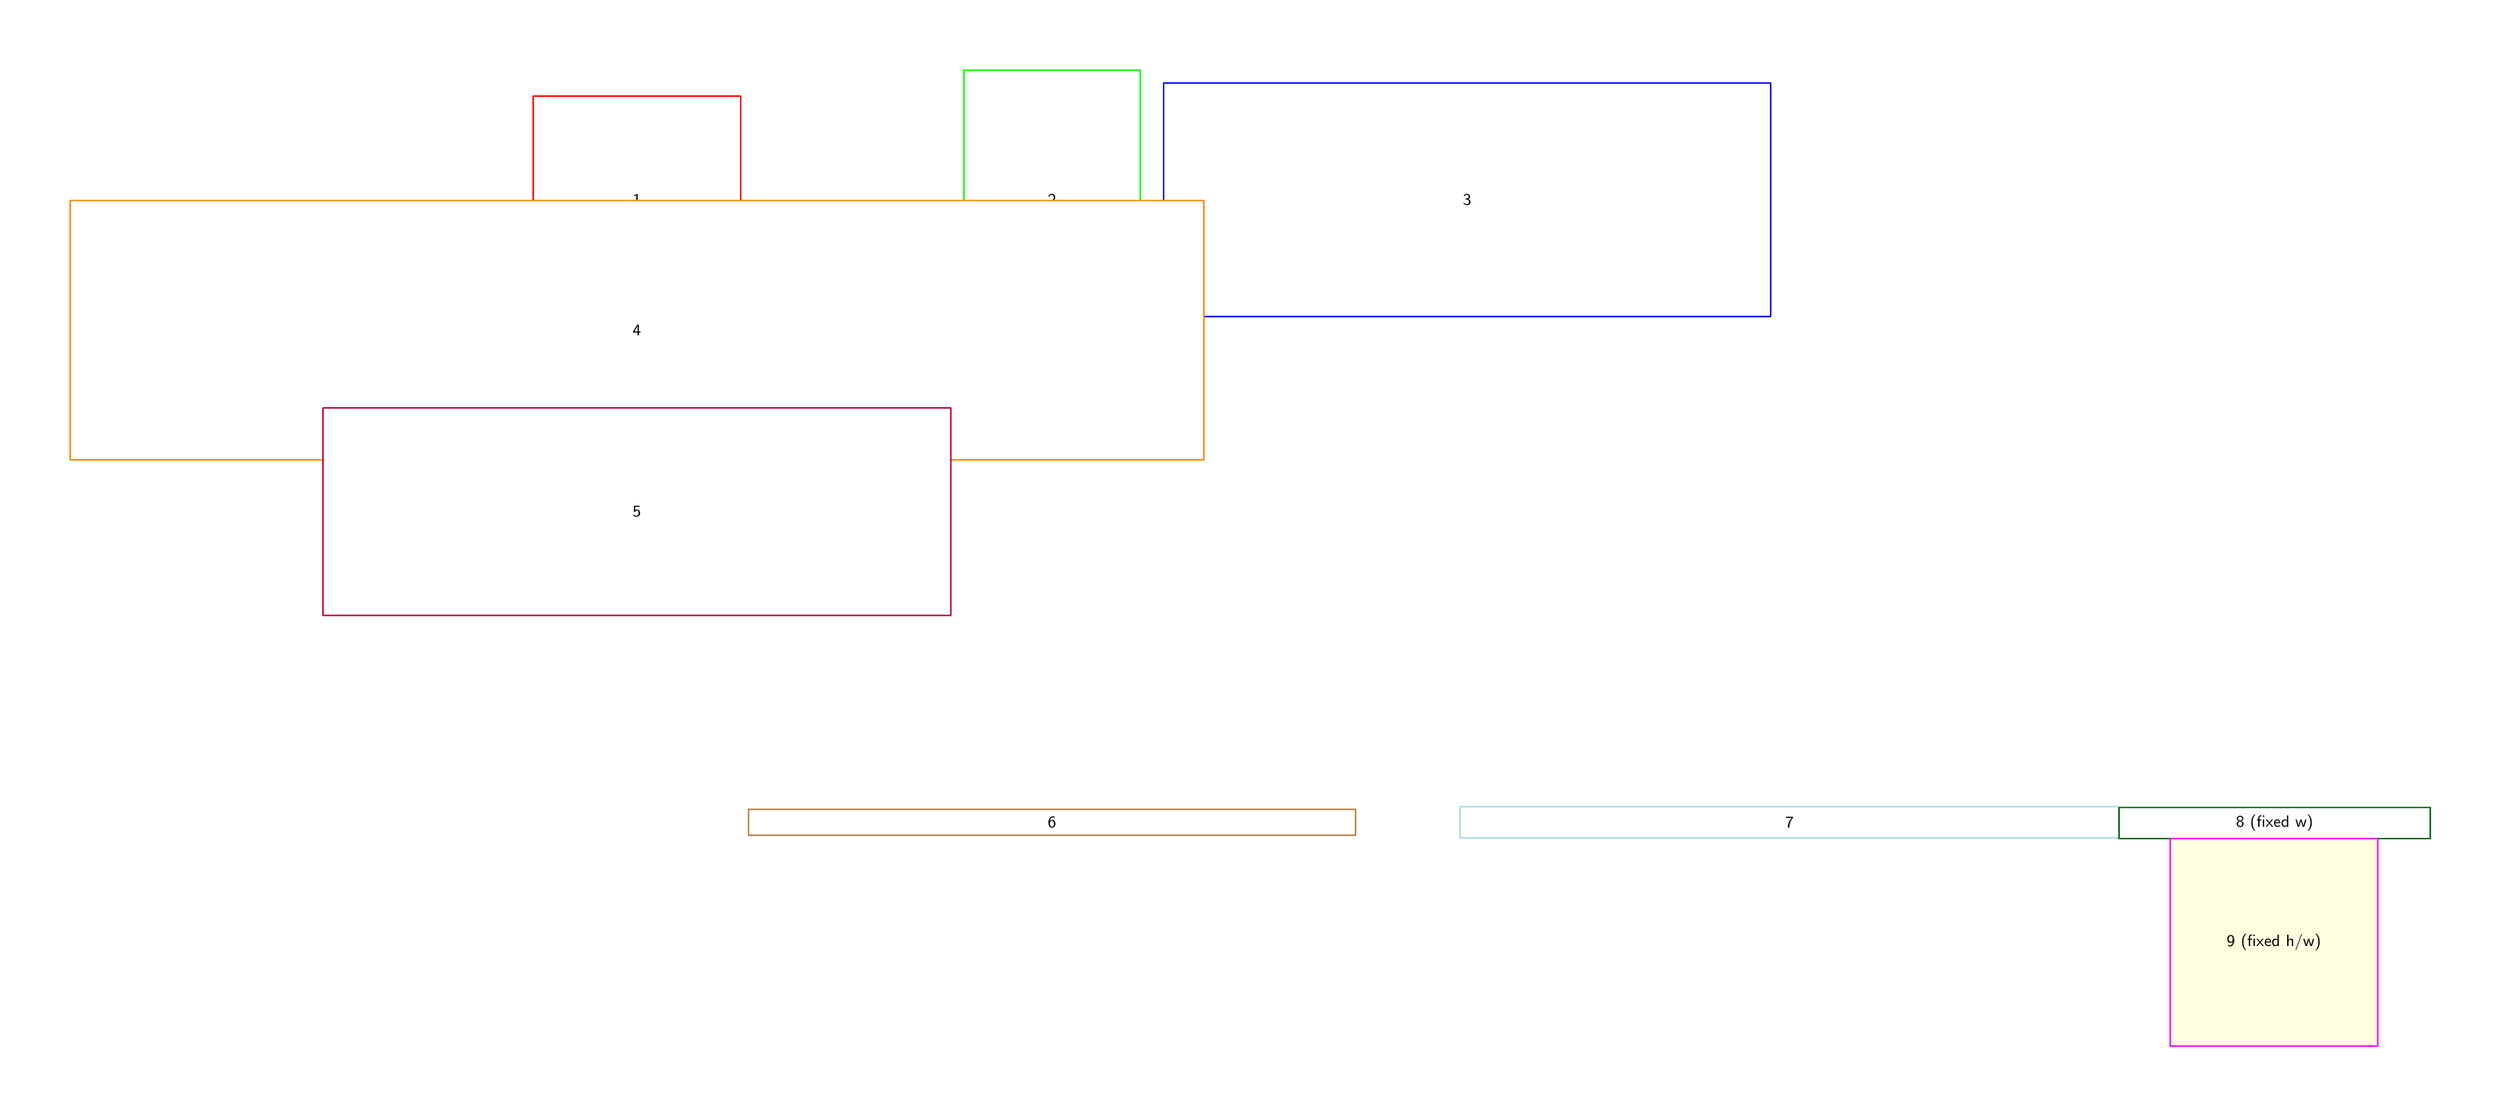
\begin{tikzpicture}
\useasboundingbox (-11.925,-17.3) rectangle (35.550000000000004,3.5);



\node[shape=rectangle, fill=colorFFFFFF, draw=red, minimum width=4cm, minimum height=4cm, rounded corners=0.005cm, line width=0.02cm, text opacity=1, font=\footnotesize, inner sep=0pt, thick] (square1) at (0,0) {\adjustbox{max width=4cm, max height=4cm}{\small{\sffamily{1}}}};
\node[shape=rectangle, fill=colorFFFFFF, draw=green, minimum width=3.4cm, minimum height=5cm, rounded corners=0.005cm, line width=0.02cm, text opacity=1, font=\footnotesize, inner sep=0pt, thick] (square2) at (8,0) {\adjustbox{max width=3.4cm, max height=5cm}{\small{\sffamily{2}}}};
\node[shape=rectangle, fill=colorFFFFFF, draw=blue, minimum width=11.7cm, minimum height=4.5cm, rounded corners=0.005cm, line width=0.02cm, text opacity=1, font=\footnotesize, inner sep=0pt, thick] (square3) at (16,0) {\adjustbox{max width=11.7cm, max height=4.5cm}{\small{\sffamily{3}}}};
\node[shape=rectangle, fill=colorFFFFFF, draw=orange, minimum width=21.85cm, minimum height=5cm, rounded corners=0.005cm, line width=0.02cm, text opacity=1, font=\footnotesize, inner sep=0pt, anchor=north, thick] (square4) at (0,0) {\adjustbox{max width=21.85cm, max height=5cm}{\small{\sffamily{4}}}};
\node[shape=rectangle, fill=colorFFFFFF, draw=purple, minimum width=12.1cm, minimum height=4cm, rounded corners=0.005cm, line width=0.02cm, text opacity=1, font=\footnotesize, inner sep=0pt, anchor=north, thick] (square5) at (0,-4) {\adjustbox{max width=12.1cm, max height=4cm}{\small{\sffamily{5}}}};
\node[shape=rectangle, fill=colorFFFFFF, draw=brown, minimum width=11.700000000000001cm, minimum height=0.5cm, rounded corners=0.005cm, line width=0.02cm, text opacity=1, font=\footnotesize, inner sep=0pt, thick] (square6) at (8,-12) {\adjustbox{max width=11.700000000000001cm, max height=0.5cm}{\small{\sffamily{6}}}};
\node[shape=rectangle, fill=colorFFFFFF, draw=LightBlue, minimum width=12.700000000000001cm, minimum height=0.6cm, rounded corners=0.005cm, line width=0.02cm, text opacity=1, font=\footnotesize, inner sep=0pt, anchor=west, thick] (square7) at (15.850000000000001,-12) {\adjustbox{max width=12.700000000000001cm, max height=0.6cm}{\small{\sffamily{7}}}};
\node[shape=rectangle, fill=colorFFFFFF, draw=DarkGreen, minimum width=6cm, minimum height=0.6cm, rounded corners=0.005cm, line width=0.02cm, text opacity=1, font=\footnotesize, inner sep=0pt, anchor=north west, thick] (square8) at (28.550000000000004,-11.7) {\adjustbox{max width=6cm, max height=0.6cm}{\small{\sffamily{8 (fixed w)}}}};
\node[shape=rectangle, fill=LightYellow, draw=Magenta, minimum width=4cm, minimum height=4cm, rounded corners=0.005cm, line width=0.02cm, text opacity=1, font=\footnotesize, inner sep=0pt, anchor=north, thick] (square9) at (31.550000000000004,-12.3) {\adjustbox{max width=4cm, max height=4cm}{\small{\sffamily{9 (fixed h/w)}}}};

\end{tikzpicture}
\end{document}